\documentclass[conference]{IEEEtran}
\IEEEoverridecommandlockouts
% The preceding line is only needed to identify funding in the first footnote. If that is unneeded, please comment it out.
%Template version as of 6/27/2024

\usepackage{cite}
\usepackage{amsmath,amssymb,amsfonts}
\usepackage{algorithmic}
\usepackage{graphicx}
\usepackage{textcomp}
\usepackage{xcolor}
\def\BibTeX{{\rm B\kern-.05em{\sc i\kern-.025em b}\kern-.08em
    T\kern-.1667em\lower.7ex\hbox{E}\kern-.125emX}}
\begin{document}

\title{Energetická optimalizácia inteligentnej budovy\\
% {\footnotesize \textsuperscript{*}Note: Sub-titles are not captured for https://ieeexplore.ieee.org  and
% should not be used}
% \thanks{Identify applicable funding agency here. If none, delete this.}
}

\author{
\IEEEauthorblockN{Bc. Lukáš Proner}
\IEEEauthorblockA{
\textit{Fakulta informatiky a elektrotechniky} \\
\textit{Technická univerzita v Košiciach} \\
Katedra počítačov a informatiky \\
Košice, Slovensko
}
\and
\IEEEauthorblockN{Bc. Peter Balog}
\IEEEauthorblockA{
\textit{Fakulta informatiky a elektrotechniky} \\
\textit{Technická univerzita v Košiciach} \\
Katedra počítačov a informatiky \\
Košice, Slovensko
}
}

\maketitle

\begin{abstract}
Prispevok sa venuje ulohe energetickej optimalizacie inteligentnej budovy na zaklade predpovedi pocasia a obsadenosti miestnosti. Zadanie odporuca vyuzit algoritmy Q-learning a DDPG a po ich implementacii porovnat ich prevadzkove vlastnosti z pohladu uspor energie oproti fixnej strategii, vplyvu roznych reward funkcii na vysledok a casu potrebneho na dosiahnutie stabilneho riesenia. Predkladany text sa zameriava primarne na vetvu riesenia zalozenu na Q-learningu, zatial co algoritmus DDPG je implementovany paralelne v ramci suvisiacej casti projektu.

\end{abstract}

\begin{IEEEkeywords}
CityLearn, energeticka optimalizacia, Q-learning, DDPG, obsadenost, predpoved pocasia, inteligentne budovy
\end{IEEEkeywords}

\section{Introduction}

Energetická optimalizácia inteligentných budov predstavuje v súčasnosti významnú výzvu, najmä z hľadiska znižovania odberu elektrickej energie zo siete, zvyšovania prevádzkovej efektívnosti a prípravy budov na pokročilé formy prediktívneho riadenia \cite{b1}.

Táto práca vychádza z konkrétne definovaného zadania, ktorého cieľom je navrhnúť a natrénovať agenta schopného optimalizovať spotrebu energie v budove na základe predpovedí počasia a informácií o obsadenosti miestností.

Ako vhodné prístupy sú uvažované algoritmy Q-learning a Deep Deterministic Policy Gradient (DDPG). Po ich implementácii budú tieto metódy porovnané z viacerých hľadísk, konkrétne z pohľadu dosiahnutých úspor energie v porovnaní s fixnou riadiacou stratégiou, citlivosti na rôzne návrhy reward funkcie a času potrebného na dosiahnutie stabilného riešenia.

\section{Špecifikácia zadania}

Zadanie s názvom \textit{Energetická optimalizácia inteligentnej budovy} je formulované ako úloha naučiť agenta využívajúceho reinforcement learning optimalizovať spotrebu energie v budove na základe predpovedí počasia a informácií o obsadenosti miestností. Ako vhodné algoritmy boli určené Q-learning a \textit{Deep Deterministic Policy Gradient} (DDPG).

Po implementácii jednotlivých prístupov majú byť ich prevádzkové vlastnosti porovnané z viacerých hľadísk:
\begin{itemize}
\item dosiahnuté úspory energie v porovnaní s fixnou riadiacou stratégiou,
\item vplyv rôznych návrhov reward funkcie na správanie agenta,
\item čas potrebný na dosiahnutie stabilného riešenia.
\end{itemize}

V praktickej rovine to znamená, že agent pracuje s vopred dostupnými informáciami, najmä s predikovanou vonkajšou teplotou, solárnym žiarením a obsadenosťou budovy, a na ich základe volí riadiace akcie vedúce k energeticky efektívnejšej prevádzke.

Z hľadiska tejto práce je dôležité zdôrazniť, že cieľom nie je iba samotné použitie metód reinforcement learningu, ale predovšetkým riešenie konkrétnej úlohy optimalizácie spotreby energie v budove, kde RL predstavuje nástroj riadenia.


\section{Prostredie CityLearn}

CityLearn predstavuje open-source simulačné prostredie určené pre reinforcement learning, zamerané na výskum koordinovaného energetického riadenia budov a mestských štvrtí. Umožňuje modelovanie jednotlivých budov spolu s ich riaditeľnými zariadeniami a energetickými subsystémami. Zároveň poskytuje štandardizované rozhranie pre definovanie observácií, akcií, odmeňovacej funkcie (reward) a vyhodnocovanie výkonnosti modelov.

Pre účely tejto práce je CityLearn obzvlášť vhodný, keďže umožňuje experimentovanie s rôznymi návrhmi reinforcement learning algoritmov v identickom simulačnom prostredí, pričom zabezpečuje konzistentný a porovnateľný spôsob ich evaluácie.

V prostredí CityLearn je každá budova reprezentovaná množinou pozorovaných veličín a množinou riaditeľných akcií. Medzi pozorovania patria napríklad predpovede počasia, solárne zisky, informácie o obsadenosti, cena elektrickej energie či aktuálne stavy energetických zásobníkov. Naopak, akčný priestor zahŕňa riadenie chladiacich systémov a v rozšírených konfiguráciách aj nabíjanie a vybíjanie tepelných alebo elektrických zásobníkov.

Ďalšou významnou výhodou prostredia CityLearn je možnosť hodnotiť výsledky pomocou interpretovateľných metrík, ako sú napríklad množstvo importovanej elektriny zo siete, kumulatívny reward či ukazovatele súvisiace s tepelným diskomfortom.

Vďaka tomu je prostredie vhodné nielen na samotný tréning agentov, ale aj na systematické porovnávanie naučených riadiacich politík s jednoduchými referenčnými stratégiami.

\section{Q-learning}

\subsection{Počiatočný návrh Q-learningu podľa zadania}

Prvá implementácia bola navrhnutá tak, aby reflektovala zadanie a využívala iba predikované vstupy, konkrétne meteorologické údaje a obsadenosť budovy. Z týchto vstupov boli vytvorené inžinierske príznaky, ako trend teploty a solárneho žiarenia či binárna informácia o obsadenosti, čo znížilo dimenzionalitu a zvýšilo ich využiteľnosť pre riadenie. Akčný priestor bol zjednodušený na riadenie chladenia s tromi diskrétnymi úrovňami, aby sa predišlo nekonzistentnosti pri absencii informácií o stave zásobníkov. Reward funkcia penalizovala odber zo siete, pričom penalizácia bola zosilnená pri obsadenej budove a vyššej teplote, čím bol agent motivovaný k opatrnejšiemu riadeniu v kritických situáciách.


\subsection{Formulácia tabuľkového Q-learningu}

Počiatočný agent využíval tabuľkový Q-learning. Stavový priestor bol diskretizovaný na konečný počet intervalov (bínov) a akčný priestor bol taktiež zredukovaný na malý počet diskrétnych hodnôt riadenia chladenia.

Q-tabuľka následne uchovávala odhady kvality vykonania konkrétnej akcie v konkrétnom diskrétnom stave. Počas tréningu agent volil akcie pomocou $\epsilon$-greedy stratégie, ktorá kombinuje exploráciu a exploitáciu.

Hodnota $\epsilon$ sa postupne znižovala, pričom bol zároveň implementovaný adaptívny mechanizmus, ktorý ju dokázal dočasne zvýšiť v prípade stagnácie učenia, teda ak nedochádzalo k zlepšovaniu výkonu agenta.

Aktualizácia hodnôt sa riadila štandardnou temporal-difference (TD) formulou:

\begin{equation}
Q(s,a) \leftarrow Q(s,a) + \alpha \left[r + \gamma \max_{a'}Q(s',a') - Q(s,a)\right]
\end{equation}

kde $s$ označuje aktuálny diskrétny stav, $a$ zvolenú akciu, $r$ prijatý reward, $s'$ nasledujúci stav, $\alpha$ mieru učenia a $\gamma$ diskontný faktor.

\subsection{Evaluácia počiatočného riešenia}

\begin{figure}[htbp]
\centerline{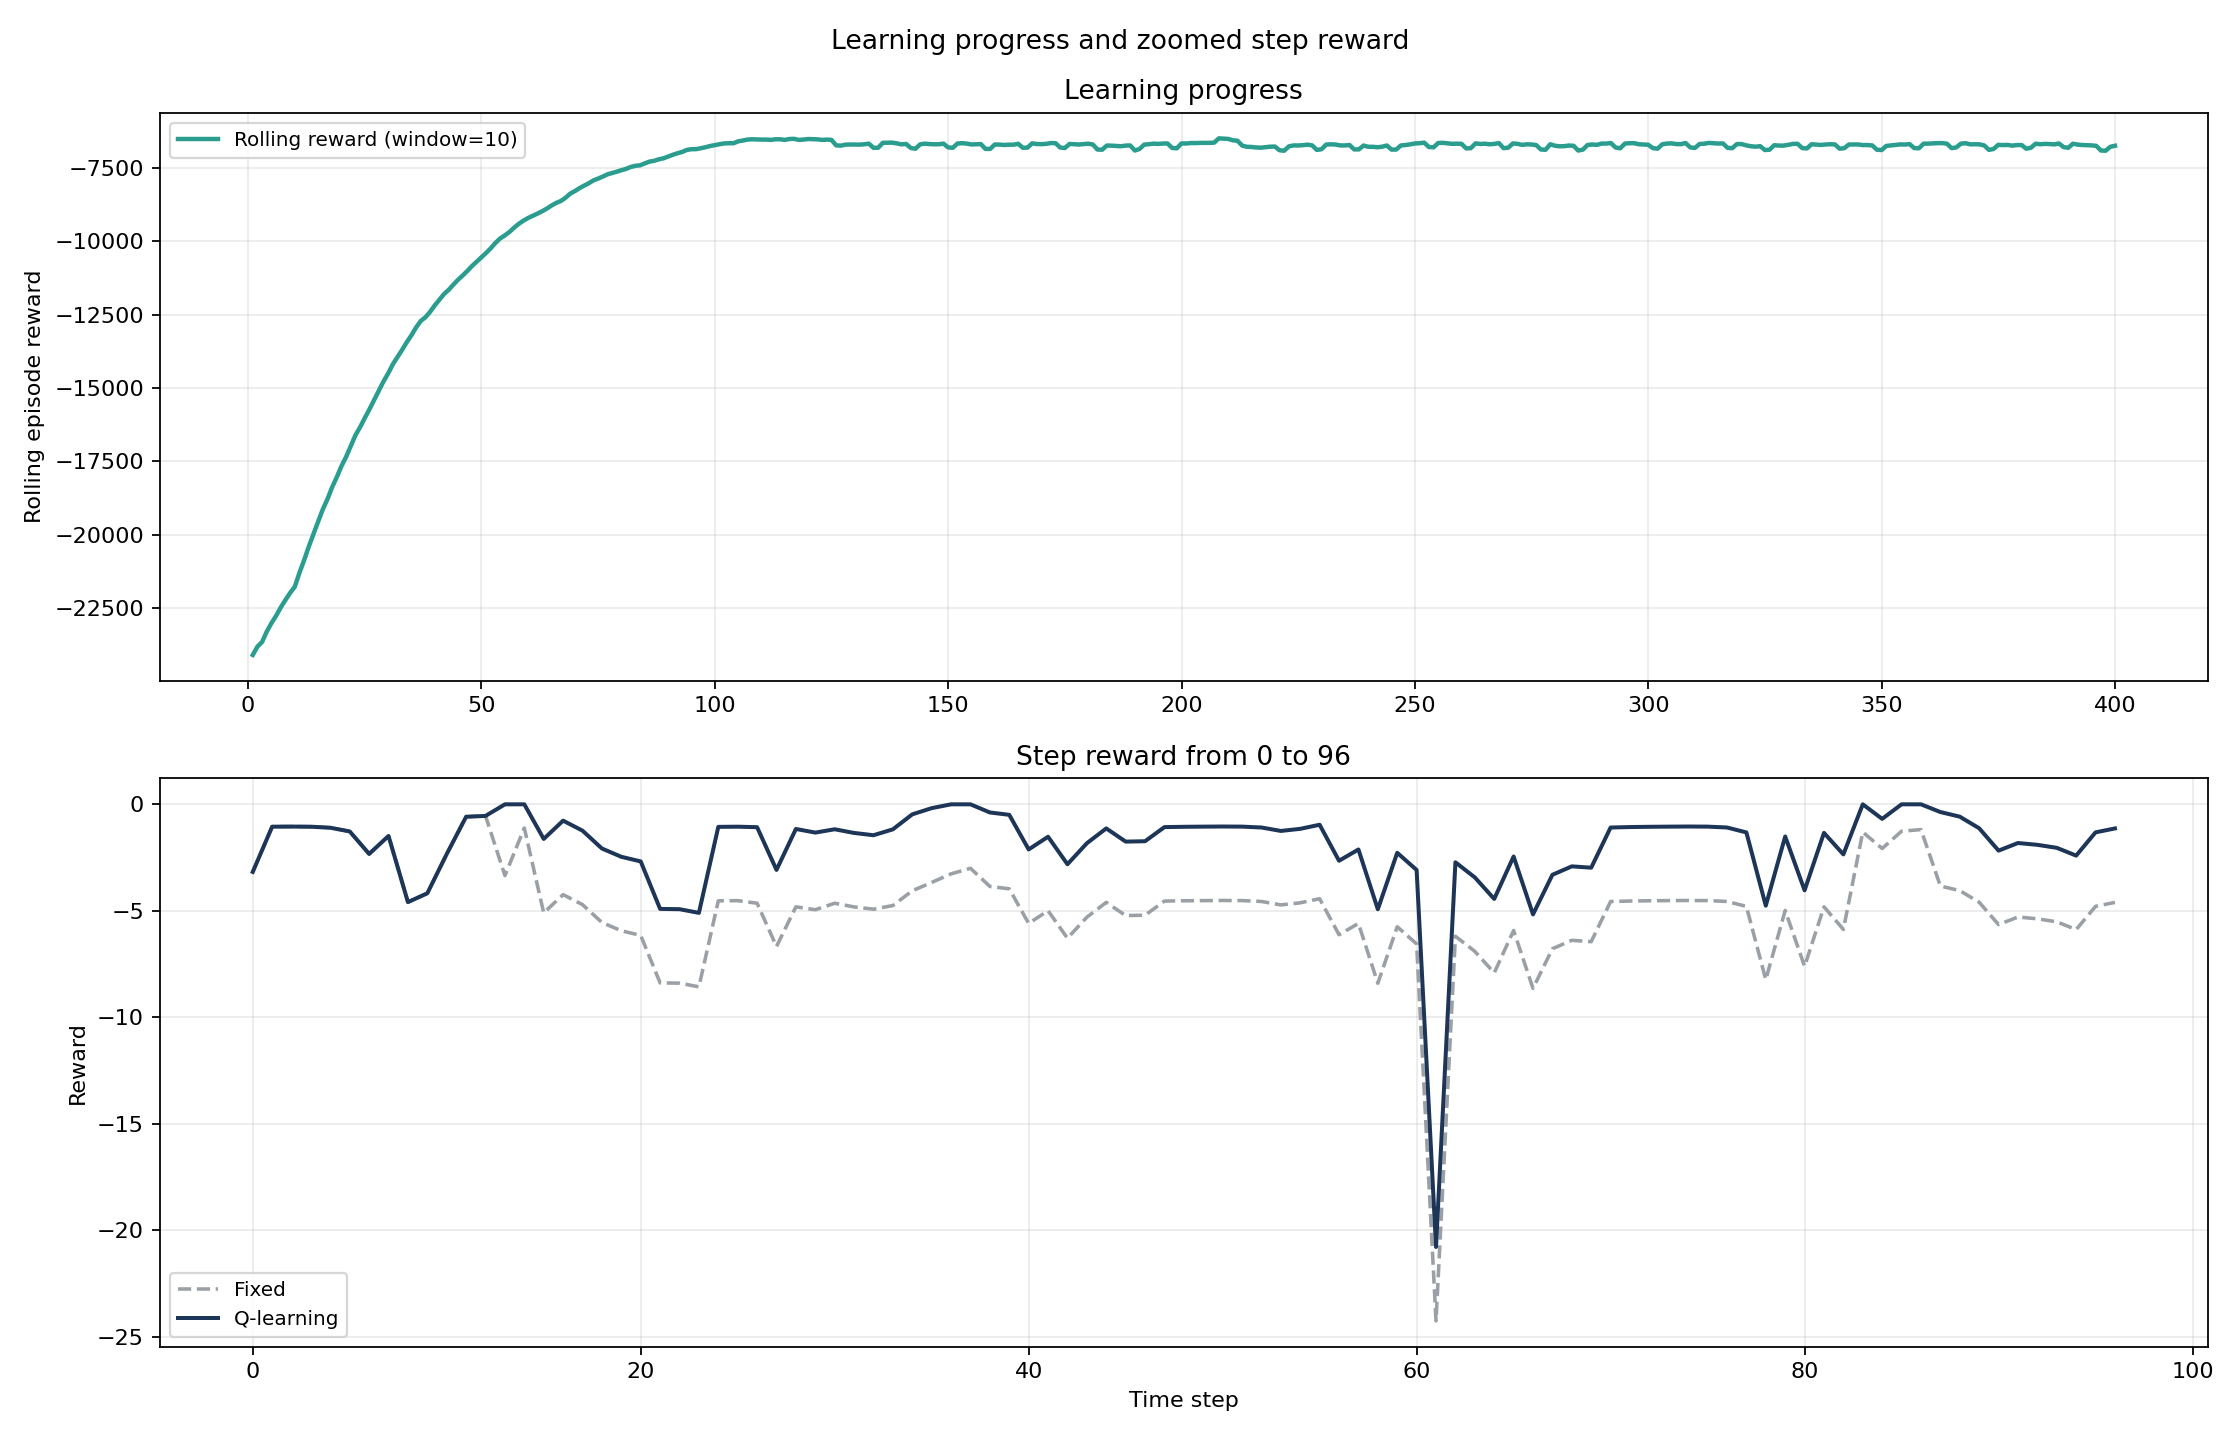
\includegraphics[width=0.4\textwidth]{learning_progress_and_step_reward_first_96_steps_weather_seed_7.png}}
\caption{Vývoj učenia a odmeny.}
\label{fig}
\end{figure}

Zo záverov vyplynulo, že model dosahoval lepšie výsledky za cenu mierne zvýšeného diskomfortu. Počiatočná formulácia síce zodpovedala zadaniu, no odhalila obmedzenia najmä v podobe príliš minimalistickej stavovej reprezentácie, ktorá nepostačuje pri rozšírení problému o ďalšie zariadenia. Rozhodovanie o zásobníkoch či reakcia na cenové signály vyžadujú dostupnosť relevantných stavových informácií. Ukazuje sa preto, že výkon agenta nezávisí len od množstva dát, ale najmä od kvality a informatívnosti stavovej reprezentácie.

\subsection{Prechod k rozšíreným Q-learning experimentom}

Po vytvorení počiatočnej verzie nasledovali rozšírené Q-learning experimenty. Stavová reprezentácia bola rozšírená o ďalšie premenné, ako cena elektriny a stav nabitia zásobníkov.

Zároveň bol rozšírený akčný priestor tak, aby zahŕňal súčasné riadenie zásobníka teplej vody, elektrického zásobníka a chladiaceho systému.

V rozšírenom experimente bolo implementovaných 12 variantov reward funkcie, ktoré menia preferencie agenta pri nezmenenom stavovom a akčnom priestore. Väčšina variantov vychádza z penalizácie odberu elektriny zo siete, pričom sa líšia v tom, aké prevádzkové priority zvýrazňujú (napr. cena elektriny, teplotný komfort alebo stav zásobníkov).

\begin{enumerate}
\item \textbf{WeatherOccupancyReward} zvyšuje penalizáciu odberu pri obsadenej budove a vyššej teplote – agent sa učí aj z rozšíreného stavového priestoru.

\item \textbf{GridImportOnlyReward} je najjednoduchší baseline $r=-g$, ktorý penalizuje iba okamžitý import zo siete bez ohľadu na cenu, komfort, predikcie či stav zásobníkov. Slúži ako referenčná politika na porovnanie zlepšenia.

\item \textbf{PricingAwareReward} rozširuje penalizáciu o cenu elektriny a podporuje presun spotreby mimo drahých období.

\item \textbf{ComfortAwareReward} kombinuje energetický a komfortný cieľ, vrátane penalizácie prehrievania.

\item \textbf{PeakShavingReward} používa kvadratickú penalizáciu $r = -g^2$, ktorá výrazne trestá špičky a vyhladzuje záťaž.

\item \textbf{SolarAlignmentReward} upravuje penalizáciu podľa slnečnej irradiácie, čím podporuje spotrebu pri vyššej produkcii obnoviteľnej energie.

\item \textbf{StorageManagementReward} pracuje so stavom zásobníkov a cenou.

\item \textbf{RampingPenaltyReward} penalizuje prudké zmeny odberu a stabilizuje profil.

\item \textbf{TimeOfUseReward} používa hodinový profil: večer vyššia penalizácia ($>1$), noc nižšia ($<1$), nezávisle od ceny a zásobníkov.

\item \textbf{SelfSufficiencyReward} penalizuje import a odmeňuje export, čím podporuje energetickú sebestačnosť.

\item \textbf{CombinedMultiObjectiveReward} kombinuje viac cieľov do váženej funkcie.

\item \textbf{NightPrechargeReward} podporuje nabíjanie v noci a vybíjanie počas špičky.
\end{enumerate}

\subsection{Equations}
Number equations consecutively. To make your 
equations more compact, you may use the solidus (~/~), the exp function, or 
appropriate exponents. Italicize Roman symbols for quantities and variables, 
but not Greek symbols. Use a long dash rather than a hyphen for a minus 
sign. Punctuate equations with commas or periods when they are part of a 
sentence, as in:
\begin{equation}
a+b=\gamma\label{eq}
\end{equation}

Be sure that the 
symbols in your equation have been defined before or immediately following 
the equation. Use ``\eqref{eq}'', not ``Eq.~\eqref{eq}'' or ``equation \eqref{eq}'', except at 
the beginning of a sentence: ``Equation \eqref{eq} is . . .''

\subsection{\LaTeX-Specific Advice}

Please use ``soft'' (e.g., \verb|\eqref{Eq}|) cross references instead
of ``hard'' references (e.g., \verb|(1)|). That will make it possible
to combine sections, add equations, or change the order of figures or
citations without having to go through the file line by line.

Please don't use the \verb|{eqnarray}| equation environment. Use
\verb|{align}| or \verb|{IEEEeqnarray}| instead. The \verb|{eqnarray}|
environment leaves unsightly spaces around relation symbols.

Please note that the \verb|{subequations}| environment in {\LaTeX}
will increment the main equation counter even when there are no
equation numbers displayed. If you forget that, you might write an
article in which the equation numbers skip from (17) to (20), causing
the copy editors to wonder if you've discovered a new method of
counting.

{\BibTeX} does not work by magic. It doesn't get the bibliographic
data from thin air but from .bib files. If you use {\BibTeX} to produce a
bibliography you must send the .bib files. 

{\LaTeX} can't read your mind. If you assign the same label to a
subsubsection and a table, you might find that Table I has been cross
referenced as Table IV-B3. 

{\LaTeX} does not have precognitive abilities. If you put a
\verb|\label| command before the command that updates the counter it's
supposed to be using, the label will pick up the last counter to be
cross referenced instead. In particular, a \verb|\label| command
should not go before the caption of a figure or a table.

Do not use \verb|\nonumber| inside the \verb|{array}| environment. It
will not stop equation numbers inside \verb|{array}| (there won't be
any anyway) and it might stop a wanted equation number in the
surrounding equation.

\subsection{Some Common Mistakes}\label{SCM}
\begin{itemize}
\item The word ``data'' is plural, not singular.
\item The subscript for the permeability of vacuum $\mu_{0}$, and other common scientific constants, is zero with subscript formatting, not a lowercase letter ``o''.
\item In American English, commas, semicolons, periods, question and exclamation marks are located within quotation marks only when a complete thought or name is cited, such as a title or full quotation. When quotation marks are used, instead of a bold or italic typeface, to highlight a word or phrase, punctuation should appear outside of the quotation marks. A parenthetical phrase or statement at the end of a sentence is punctuated outside of the closing parenthesis (like this). (A parenthetical sentence is punctuated within the parentheses.)
\item A graph within a graph is an ``inset'', not an ``insert''. The word alternatively is preferred to the word ``alternately'' (unless you really mean something that alternates).
\item Do not use the word ``essentially'' to mean ``approximately'' or ``effectively''.
\item In your paper title, if the words ``that uses'' can accurately replace the word ``using'', capitalize the ``u''; if not, keep using lower-cased.
\item Be aware of the different meanings of the homophones ``affect'' and ``effect'', ``complement'' and ``compliment'', ``discreet'' and ``discrete'', ``principal'' and ``principle''.
\item Do not confuse ``imply'' and ``infer''.
\item The prefix ``non'' is not a word; it should be joined to the word it modifies, usually without a hyphen.
\item There is no period after the ``et'' in the Latin abbreviation ``et al.''.
\item The abbreviation ``i.e.'' means ``that is'', and the abbreviation ``e.g.'' means ``for example''.
\end{itemize}
An excellent style manual for science writers is \cite{b7}.

\subsection{Authors and Affiliations}\label{AAA}
\textbf{The class file is designed for, but not limited to, six authors.} A 
minimum of one author is required for all conference articles. Author names 
should be listed starting from left to right and then moving down to the 
next line. This is the author sequence that will be used in future citations 
and by indexing services. Names should not be listed in columns nor group by 
affiliation. Please keep your affiliations as succinct as possible (for 
example, do not differentiate among departments of the same organization).

\subsection{Identify the Headings}\label{ITH}
Headings, or heads, are organizational devices that guide the reader through 
your paper. There are two types: component heads and text heads.

Component heads identify the different components of your paper and are not 
topically subordinate to each other. Examples include Acknowledgments and 
References and, for these, the correct style to use is ``Heading 5''. Use 
``figure caption'' for your Figure captions, and ``table head'' for your 
table title. Run-in heads, such as ``Abstract'', will require you to apply a 
style (in this case, italic) in addition to the style provided by the drop 
down menu to differentiate the head from the text.

Text heads organize the topics on a relational, hierarchical basis. For 
example, the paper title is the primary text head because all subsequent 
material relates and elaborates on this one topic. If there are two or more 
sub-topics, the next level head (uppercase Roman numerals) should be used 
and, conversely, if there are not at least two sub-topics, then no subheads 
should be introduced.

\subsection{Figures and Tables}\label{FAT}
\paragraph{Positioning Figures and Tables} Place figures and tables at the top and 
bottom of columns. Avoid placing them in the middle of columns. Large 
figures and tables may span across both columns. Figure captions should be 
below the figures; table heads should appear above the tables. Insert 
figures and tables after they are cited in the text. Use the abbreviation 
``Fig.~\ref{fig}'', even at the beginning of a sentence.

\begin{table}[htbp]
\caption{Table Type Styles}
\begin{center}
\begin{tabular}{|c|c|c|c|}
\hline
\textbf{Table}&\multicolumn{3}{|c|}{\textbf{Table Column Head}} \\
\cline{2-4} 
\textbf{Head} & \textbf{\textit{Table column subhead}}& \textbf{\textit{Subhead}}& \textbf{\textit{Subhead}} \\
\hline
copy& More table copy$^{\mathrm{a}}$& &  \\
\hline
\multicolumn{4}{l}{$^{\mathrm{a}}$Sample of a Table footnote.}
\end{tabular}
\label{tab1}
\end{center}
\end{table}

\begin{figure}[htbp]
\centerline{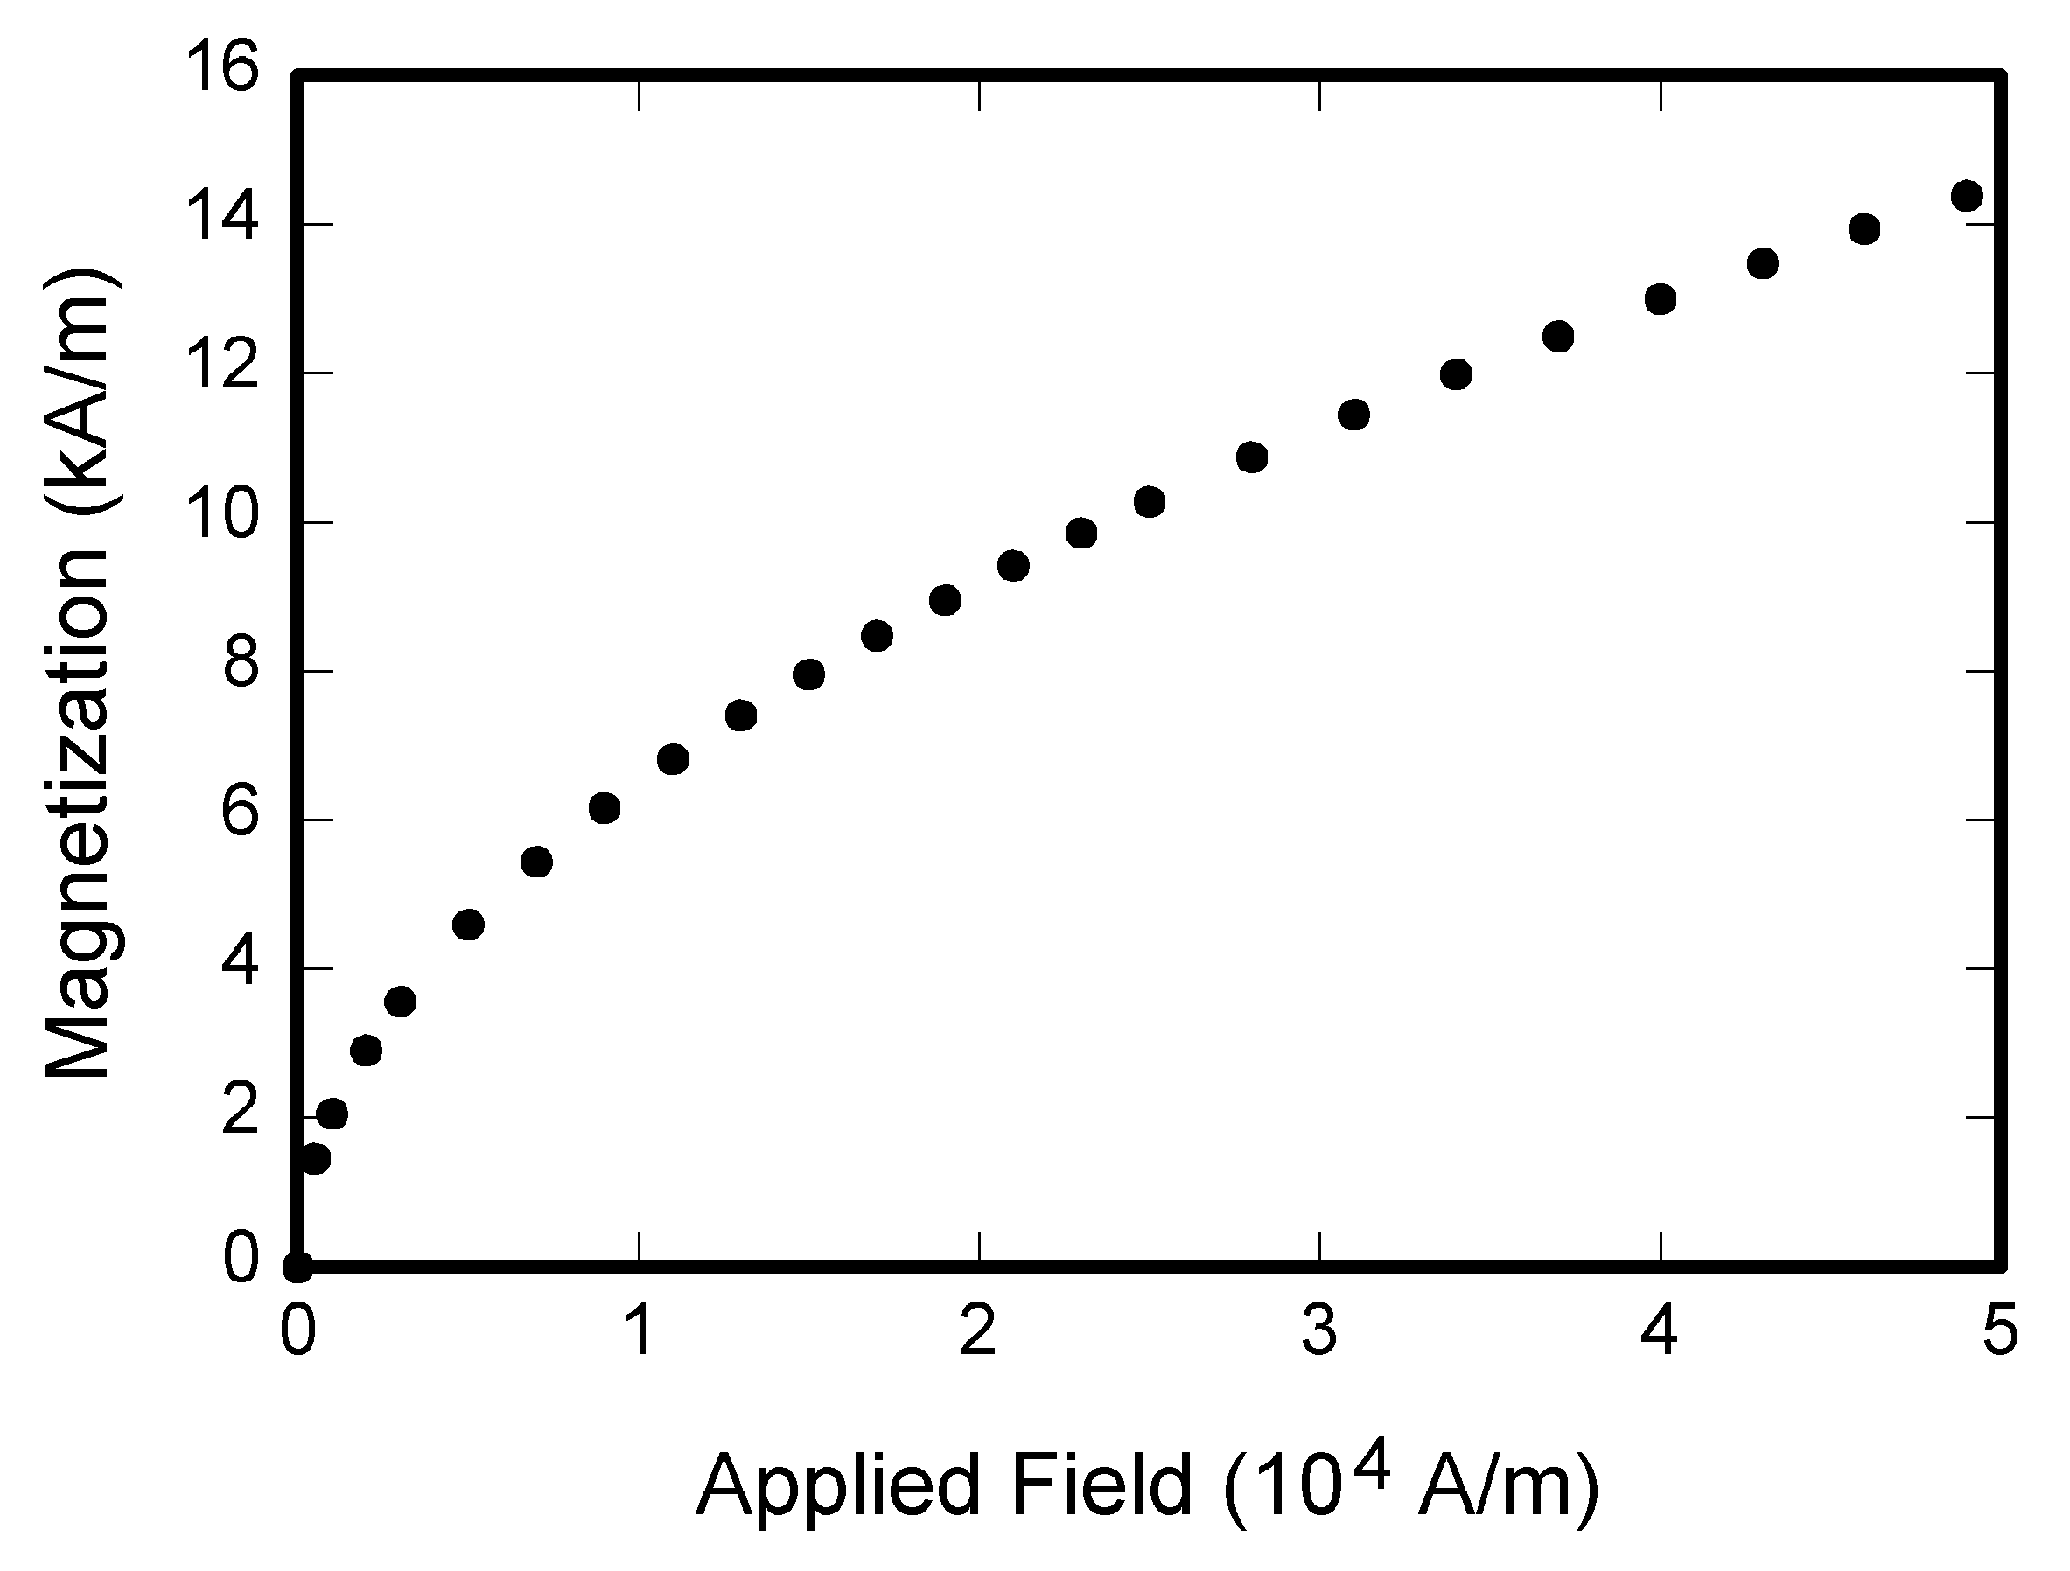
\includegraphics{fig1.png}}
\caption{Example of a figure caption.}
\label{fig}
\end{figure}

Figure Labels: Use 8 point Times New Roman for Figure labels. Use words 
rather than symbols or abbreviations when writing Figure axis labels to 
avoid confusing the reader. As an example, write the quantity 
``Magnetization'', or ``Magnetization, M'', not just ``M''. If including 
units in the label, present them within parentheses. Do not label axes only 
with units. In the example, write ``Magnetization (A/m)'' or ``Magnetization 
\{A[m(1)]\}'', not just ``A/m''. Do not label axes with a ratio of 
quantities and units. For example, write ``Temperature (K)'', not 
``Temperature/K''.

\section*{Acknowledgment}

The preferred spelling of the word ``acknowledgment'' in America is without 
an ``e'' after the ``g''. Avoid the stilted expression ``one of us (R. B. 
G.) thanks $\ldots$''. Instead, try ``R. B. G. thanks$\ldots$''. Put sponsor 
acknowledgments in the unnumbered footnote on the first page.

\section*{References}

Please number citations consecutively within brackets \cite{b1}. The 
sentence punctuation follows the bracket \cite{b2}. Refer simply to the reference 
number, as in \cite{b3}---do not use ``Ref. \cite{b3}'' or ``reference \cite{b3}'' except at 
the beginning of a sentence: ``Reference \cite{b3} was the first $\ldots$''

Number footnotes separately in superscripts. Place the actual footnote at 
the bottom of the column in which it was cited. Do not put footnotes in the 
abstract or reference list. Use letters for table footnotes.

Unless there are six authors or more give all authors' names; do not use 
``et al.''. Papers that have not been published, even if they have been 
submitted for publication, should be cited as ``unpublished'' \cite{b4}. Papers 
that have been accepted for publication should be cited as ``in press'' \cite{b5}. 
Capitalize only the first word in a paper title, except for proper nouns and 
element symbols.

For papers published in translation journals, please give the English 
citation first, followed by the original foreign-language citation \cite{b6}.

\begin{thebibliography}{00}
\bibitem{b1} J. R. Vázquez-Canteli, Z. Nagy, S. Dey, and G. Henze, 
``CityLearn: Standardizing Research in Multi-Agent Reinforcement Learning for Demand Response and Urban Energy Management,'' 
The University of Texas at Austin and University of Colorado Boulder.
\bibitem{b2} J. Clerk Maxwell, A Treatise on Electricity and Magnetism, 3rd ed., vol. 2. Oxford: Clarendon, 1892, pp.68--73.
\bibitem{b3} I. S. Jacobs and C. P. Bean, ``Fine particles, thin films and exchange anisotropy,'' in Magnetism, vol. III, G. T. Rado and H. Suhl, Eds. New York: Academic, 1963, pp. 271--350.
\bibitem{b4} K. Elissa, ``Title of paper if known,'' unpublished.
\bibitem{b5} R. Nicole, ``Title of paper with only first word capitalized,'' J. Name Stand. Abbrev., in press.
\bibitem{b6} Y. Yorozu, M. Hirano, K. Oka, and Y. Tagawa, ``Electron spectroscopy studies on magneto-optical media and plastic substrate interface,'' IEEE Transl. J. Magn. Japan, vol. 2, pp. 740--741, August 1987 [Digests 9th Annual Conf. Magnetics Japan, p. 301, 1982].
\bibitem{b7} M. Young, The Technical Writer's Handbook. Mill Valley, CA: University Science, 1989.
\bibitem{b8} D. P. Kingma and M. Welling, ``Auto-encoding variational Bayes,'' 2013, arXiv:1312.6114. [Online]. Available: https://arxiv.org/abs/1312.6114
\bibitem{b9} S. Liu, ``Wi-Fi Energy Detection Testbed (12MTC),'' 2023, gitHub repository. [Online]. Available: https://github.com/liustone99/Wi-Fi-Energy-Detection-Testbed-12MTC
\bibitem{b10} ``Treatment episode data set: discharges (TEDS-D): concatenated, 2006 to 2009.'' U.S. Department of Health and Human Services, Substance Abuse and Mental Health Services Administration, Office of Applied Studies, August, 2013, DOI:10.3886/ICPSR30122.v2
\bibitem{b11} K. Eves and J. Valasek, ``Adaptive control for singularly perturbed systems examples,'' Code Ocean, Aug. 2023. [Online]. Available: https://codeocean.com/capsule/4989235/tree
\end{thebibliography}

\vspace{12pt}
\color{red}
IEEE conference templates contain guidance text for composing and formatting conference papers. Please ensure that all template text is removed from your conference paper prior to submission to the conference. Failure to remove the template text from your paper may result in your paper not being published.

\end{document}
